\section{Networking between a host and the players}
The following section will examine the different possibilities regarding transmitting player position data to the Unity application.

\subsection{Possible solutions}
Unity will be used for the creation of the game aspect of this project as described in \todo{ref til Unity section}.
Unity includes a proprietary networking solution known as UNet\cite{unityunet}.
This solution allows developers to use a high-level API, giving access to commands that cover many common requirements for multiplayer games, without worrying about the low-level details.
Since the solution is developed alongside the actual game engine, it has a higher level of integration with the Unity Editor and Engine, which allows for certain components and visual aids to aid the building of the game.
As of the beginning of this project, the UNet solution has been deprecated for a while, and the Unity developers are actively working to create a new system to replace it.
The current UNet iteration is usable, but will be removed in the future.
Other third-party solutions for Unity based games also exist, such as Photon Engine.
Photon provides functionality for the developers to make use of in order to create multiplayer games in the same way as UNet, exposing higher-level functionality.
Photon supports multiple platforms outside of just Unity, with both Android and iOS support \cite{photonnet}.
\\\\
The alternative to making use of a pre-existing solution is creating a custom solution.
SOCKETS??
UNDERSØG WINDOWS COMMUNICATION FOUNDATION - WCF??
\subsection{Choosing a solution}
There are certain pros and cons associated with both approaches of using either a pre-existing solution or a custom solution.
\autoref{tab:networksolprosandcons} 
\begin{table}[]
    \begin{tabular}{|l|l|l|}
    \hline
                    & Pre-existing                                                & Custom                                                                            \\ \hline
    Customizability & Consists of a set of pre-defined functionalities            & Can have any functionality implemented                                            \\ \hline
    Requirements    & Familiarity with the solution                               & Familiarity with the knowledge required to implement a usable solution            \\ \hline
    Optimization    & Lower-level details are obscured, optimized for general use & Lower-level details are freely available, can be optimized for a specific purpose \\ \hline
    \end{tabular}
    \caption{A comparison of the pros and cons of the possible solutions}
    \label{tab:networksolprosandcons}
    \end{table}

\subsection{Introduction to sockets}
LAV OG INDSÆT BILLEDE AF OSI LAYER OG HVOR SOCKETS ER :D
Programs that communicate across a computer network need an agreement on how those programs will communicate.
This is known as a protocol.

\begin{figure}[H]
    \centering
    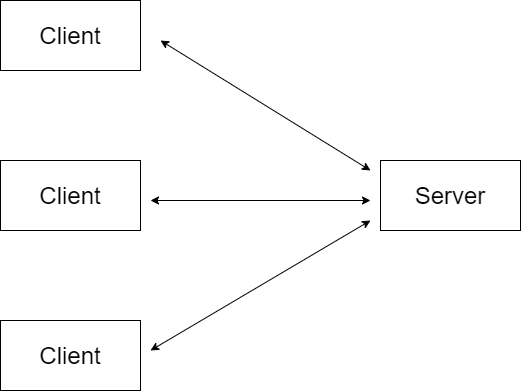
\includegraphics[width=0.6\linewidth]{client_server.png}
    \caption{An illustration of the client-server architecture}
    \label{fig:client-server}
\end{figure}

